\section{Maturing Legal RAG Systems and Evaluation Research (2025)}
\label{sec:maturing}

Where 2024 established the problem of legal RAG and the metrics needed to evaluate it, 2025 is the
year complete systems and larger-scale evaluation studies arrived. This section follows eleven
studies from that year, organized into two groups: deployed or applied legal RAG systems, and the
evaluation, reliability, and survey literature that assessed them.

\subsection{Legal RAG applications}

\citet{buffa2025} published \textbf{JusBuild}, a system for drafting structured legal documents. It
segments existing documents into functional sections, retrieves relevant precedent sections during
drafting, and offers AI-generated suggestions while keeping a human professional in control of the
final formulation, shown in Figure~\ref{fig:jusbuild}. The authors evaluated JusBuild across datasets
that differ in language, template, and judicial matter. Its central design choice, keeping a human
in the loop rather than generating a final document on its own, reflects a judgment this survey
returns to directly in Section~\ref{sec:reliability}: retrieval-augmented drafting reduces, but does
not eliminate, the need for professional review.

% Figure reproduced from Buffa et al. (2025), "Enhancing legal document building with
% Retrieval-Augmented Generation" (Computer Law & Security Review), Fig. 1, for scholarly
% discussion and critique within this review. Copyright remains with the original
% authors/publisher.
\begin{figure*}[t]
\centering
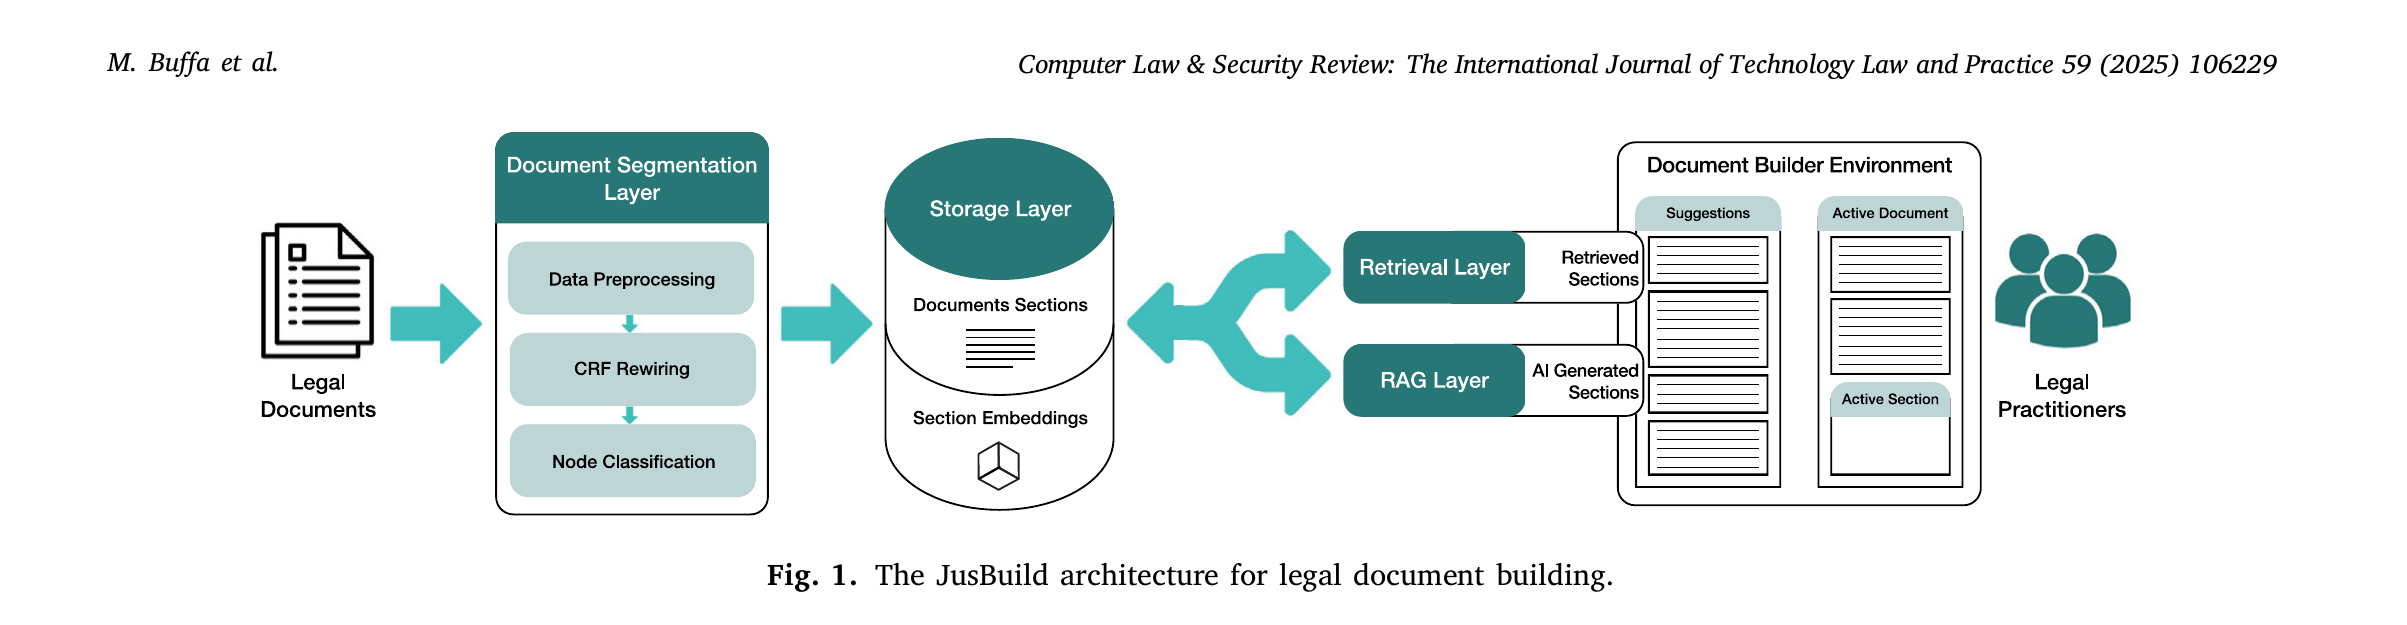
\includegraphics[width=\textwidth]{images/buffa2025_fig1.png}
\caption{Figure reproduced from \citet{buffa2025}: the JusBuild architecture for legal document
building. Legal documents pass through a Document Segmentation Layer (preprocessing, CRF
rewiring, node classification) into a Storage Layer of document sections and their embeddings.
At drafting time, a Retrieval Layer returns relevant retrieved sections and a RAG Layer returns
AI-generated sections, both surfaced to the legal practitioner inside the Document Builder
Environment alongside the document currently being drafted.}
\label{fig:jusbuild}
\end{figure*}


In the same year, \citet{zhang2025} proposed a multi-round RAG approach to comprehensive legal
document analysis. It retrieves evidence iteratively across several rounds instead of in a single
pass, which helps with questions no single retrieval step can resolve. \citet{ref312025} then
applied legal RAG to a jurisdiction this survey gives particular attention to: Pakistan. Their
framework combines semantic and keyword-based retrieval over selected Pakistani legal materials,
including the Code of Criminal Procedure and the Pakistan Penal Code. It shows concretely why
jurisdiction-specific evidence, not just a capable retrieval method, matters for legal question
answering. Section~\ref{sec:jurisdiction} examines this jurisdiction in depth, alongside the 2026
system that extends this line of work.

\subsection{Evaluation, reliability, and the surrounding survey literature}

The remaining 2025 studies turned attention from building legal RAG systems to assessing them, and
to surveying the field itself. \citet{premasiri2025} surveyed legal information extraction broadly.
They pulled together the extraction-focused line of work this survey traced from
\citet{chalkidis2017} in Section~\ref{sec:outcomes} through the knowledge-graph systems in
Section~\ref{sec:lm2023}. \citet{magesh2025} then directly tested the hallucination question
\citet{dahl2024} had raised the previous year. They assessed several leading commercial AI legal
research tools and found that hallucinations persisted despite those tools' use of
retrieval-augmented generation. This challenges any assumption that adding retrieval alone
guarantees a hallucination-free system. \citet{kelsall2025} carried out a rapid evidence review of
evaluation techniques for large language models in legal use cases. They found persistent gaps in
how researchers design and report legal AI evaluations. \citet{benedetto2025} proposed
\textbf{LR2}, a legal RAG system built specifically for legal reasoning over case law, and
\citet{italiani2025} looked at data generation and knowledge distillation as a way to improve legal
question answering without needing a full-scale retrieval pipeline for every deployment.
\citet{dugac2025} studied the harder problem of classifying legal \emph{interpretations} with large
language models. This is a more demanding task than classifying legal text by topic, because it
requires telling apart competing readings of the same provision. \citet{kim2025} stepped back from
individual systems to prioritize the challenges facing AI adoption in the legal domain more broadly.
They combined a systematic review with an expert-driven analytic hierarchy process. Finally,
\citet{tritto2025} surveyed causal artificial intelligence in legal language processing. They
pointed toward a research direction the systems discussed so far in this survey do not yet address:
reasoning about cause and effect instead of pattern similarity.

Read together, this year's studies show a field moving from asking whether legal RAG works in
principle to asking, with increasing precision, where specifically it fails and for whom. That
question motivates the final year of this survey's chronological account, 2026, where we situate
this survey's own comparative case study.
